% additional use of \usepackage{beamerthemesplit}
\documentclass{beamer}
\usepackage{beamerthemesplit} % new 
\usepackage{hyperref}
\usepackage{multimedia}
\usepackage[spanish]{babel}
\usetheme{Frankfurt}
\definecolor{verde}{rgb}{0,0,1}
\definecolor{rojo}{rgb}{1,0,0}
\definecolor{vio}{rgb}{0.5,0,0.5}
\definecolor{rosa}{rgb}{0.8,0.1,0.1}
\newcommand{\director}{Directores:\\ Mariano Dominguez \& Dante Paz}

\begin{document}
\title{Cat\'alogo de c\'umulos de galaxias en proceso de fusi\'on.} 
\author{Mart\'in de los Rios}

\frame{\titlepage

\director
} 

\frame{
\tableofcontents} 


\section{Motivaciones.}
\frame{
\tableofcontents[ 
    currentsection, 
    hideothersections, 
    sectionstyle=show/hide, 
    sectionstyle=show/shaded, 
    ] 
}

\frame{\frametitle{ Motivaciones}
\begin{itemize}
 \item El estudio de la din\'amica de los c\'umulos en colisi\'on permite determinar algunas propiedades de la part\'icula de materia oscura.
\end{itemize}

}


\frame{\frametitle{Sistemas virializados}
\begin{itemize}
 \item Masa estimada a partir de la din\'amica.
\end{itemize}

\begin{figure}[h!]
\begin{tabular}{cc}

 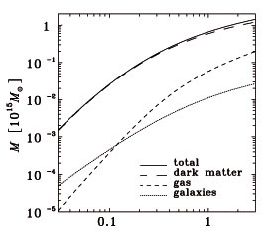
\includegraphics[bb=0 0 132 111,scale=1]{./Lokas1.pdf}& 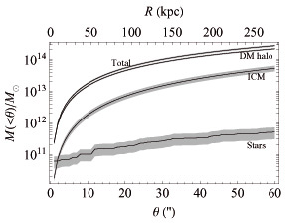
\includegraphics[scale=1]{./Sereno.pdf}\\
 Cumulo de coma  & Cumulo AC 114 \\
 Lokas et al. 2003 & Sereno et al. 2008
\end{tabular}
\end{figure}

}


\frame{\frametitle{Curvas de rotaci\'on de galaxias espirales}
\begin{figure}[h!]
 \centering
 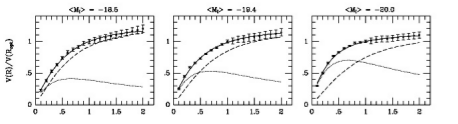
\includegraphics[scale=0.8]{./Simbre.png}
 \caption{Salucci et al. (2007)}
 % Salucci.pdf: 340x387 pixel, 72dpi, 11.99x13.65 cm, bb=0 0 340 387
\end{figure}

}

\frame{\frametitle{Lentes gravitacionales}
\begin{itemize}
 \item Masa estimada a partir de las deformaciones producidas por las lentes gravitacionales.
\end{itemize}

\begin{figure}[h!]
 \centering
 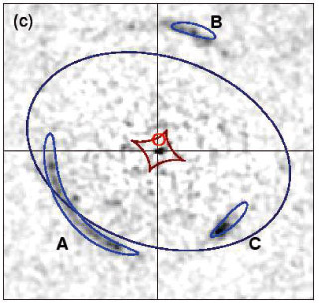
\includegraphics[bb=0 0 153 146,scale=0.8]{./Smith.pdf}
 \caption{Smith et al. (2005)}
 % Smith.pdf: 153x146 pixel, 72dpi, 5.40x5.15 cm, bb=0 0 153 146
\end{figure}

}


\frame{\frametitle{Fondo c\'osmico de microondas}
\begin{itemize}
 \item A trav\'es del ajuste los multipolos se pueden estimar algunos par\'ametros cosmol\'ogicos, como por ejemplo la densidad de materia.
\end{itemize}

\begin{figure}[!]
\begin{tabular}{cc}

 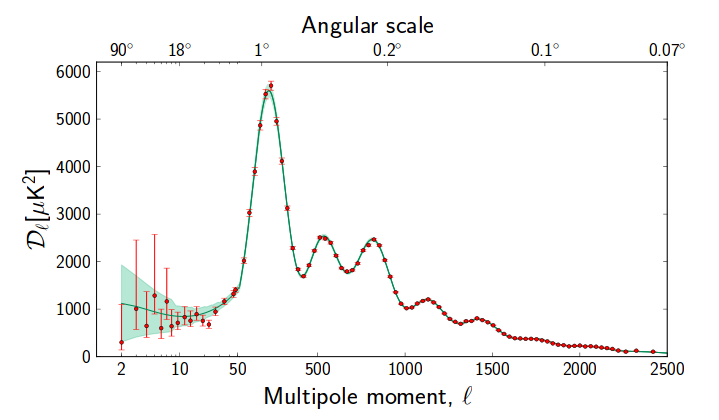
\includegraphics[scale=0.22]{./planck.png} & 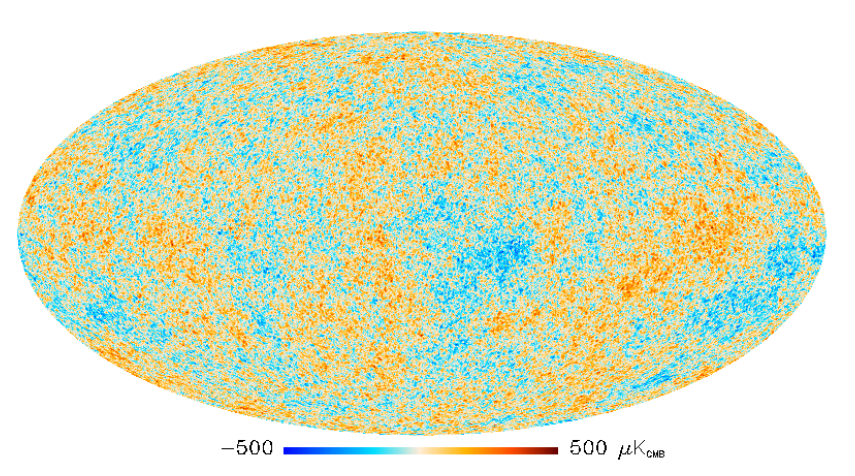
\includegraphics[scale=0.18]{./cmb.png}
  
\end{tabular}
\caption{Planck collaboration 2013}
\end{figure}

}


\frame{\frametitle{Modelo cosmol\'ogico est\'andar.}
\begin{figure}[h!]

 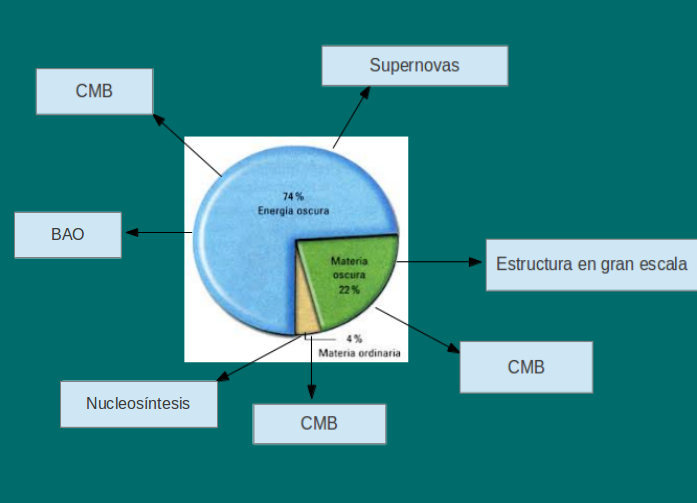
\includegraphics[scale=0.45]{./torta2.png}
 
\end{figure}

}


\frame{ \frametitle{Estrategias de detecci\'on de materia oscura.}
\begin{figure}[h!]
 \centering
 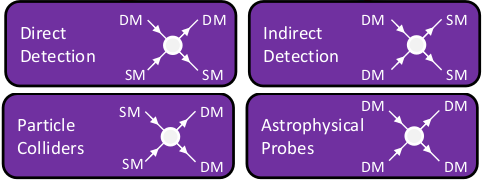
\includegraphics[scale=0.4]{./busqueda2.png}
 % busqueda2.png: 489x184 pixel, 72dpi, 17.25x6.49 cm, bb=0 0 489 184
\end{figure}
\begin{itemize}
 \item Estudiando la emisi\'on de rayos-$\gamma$ de diferentes fuentes astrof\'isicas (Galaxia Andr\'omeda, C\'umulo de Coma,etc.) se identific\'o
 una l\'inea de emisi\'on en $E=3.55 \pm 0.03 Kev$, que puede ser interpretada como la emisi\'on producida por el decaimiento de un neutrino est\'eril
 con una masa de $m_{sn}=7.06 \pm 0.05 Kev$. \textit{Boyarsky et al.} y \textit{Bulbuk et al.}.
 \item Esta interpretaci\'on es consistente con todos los l\'imites provenientes de otras observaciones cosmol\'ogicas.
\end{itemize}

}

\subsection{Bullet cluster} 

\frame{\frametitle{The Bullet Cluster}
\begin{tiny}
\begin{columns}
 \begin{column}{4cm}
  \begin{itemize}
  \item Imagen en el \'optico.
   \item {\color{rosa} Emisi\'on en rayos x.}
   \item {\color{vio} Masa estimada por LG.}
  \end{itemize}
 \end{column}
\begin{column}{7cm}
\begin{figure}
 \centering
 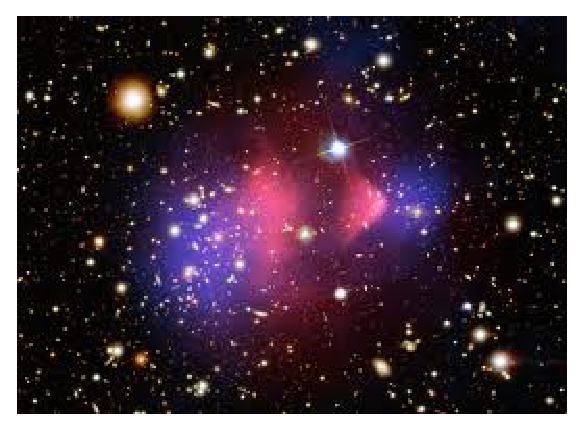
\includegraphics[scale=0.8]{./bullet.eps}
\end{figure}
\end{column}
\end{columns}
\end{tiny}

\href{run:bullet.avi}{video}

}

\frame{\frametitle{Bullet Cluster}
\begin{figure}[!b]
 \centering
 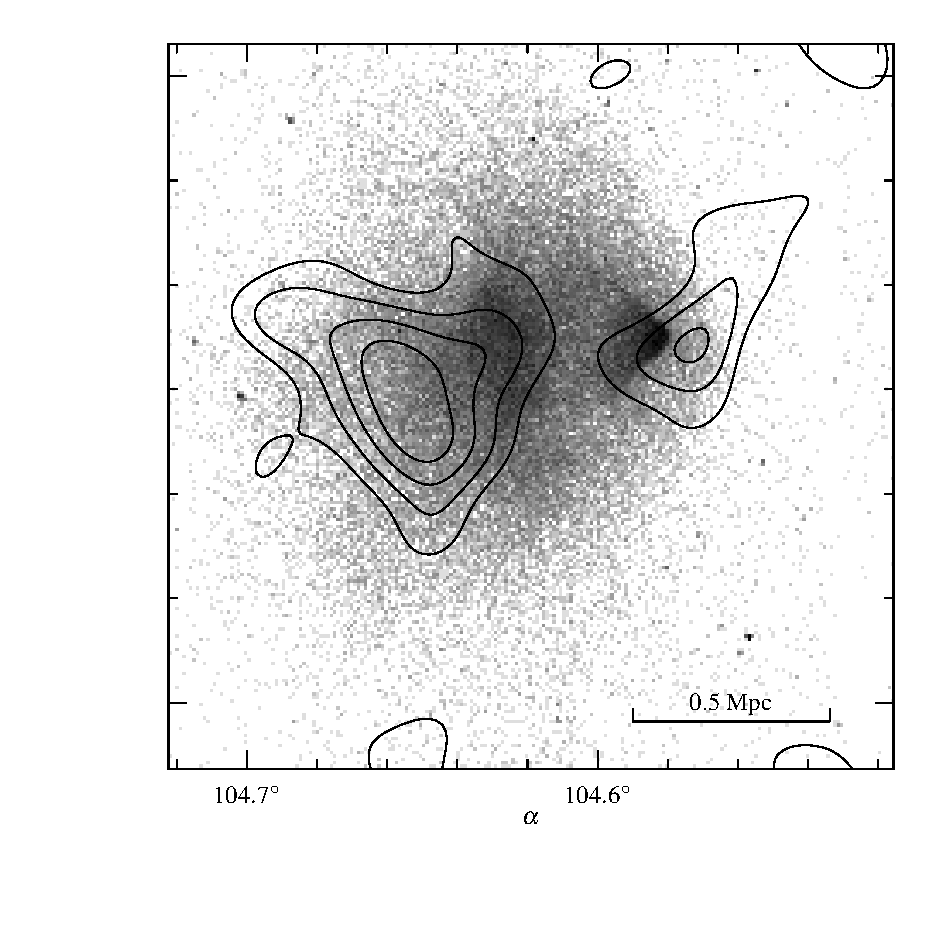
\includegraphics[scale=0.25]{./1e_xrayimg_lens_sm7.eps}
 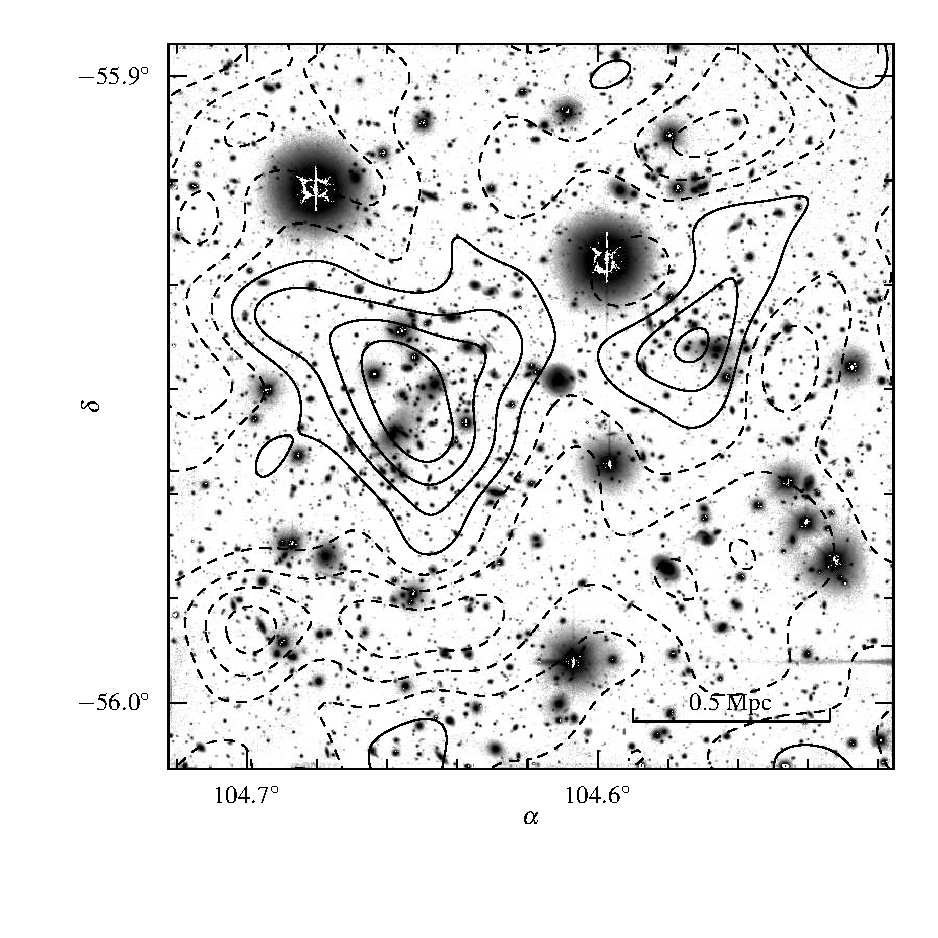
\includegraphics[scale=0.25]{./1e_optvlt_lens_sm7.eps}
 % 1e_optvlt_lens_sm7.eps: 0x0 pixel, 300dpi, 0.00x0.00 cm, bb=0 0 434 434
\end{figure}
}
\frame{\frametitle{Markevitch et al. 2004}
\begin{itemize}
 \item Desfasaje entre la materia oscura y el gas:
\end{itemize}

$ \tau_{s}=\frac{\sigma}{m} \Sigma_{s} $ 
donde $\sigma$ es la secci\'on eficaz, \textit{m} es la masa de la part\'icula y $\Sigma_{s}$ es la densidad superficial de DM.
La densidad superficial promediada dentro de $r = r_{tr}$ es $\Sigma \approx 0.2 g cm^{-2}$,
entonces, asumiendo simetr\'ia esf\'erica y pidiendo que $\tau_{s}<1$ tenemos: $\frac{\sigma}{m} < 5 cm^{2}g^{-1}$.

\begin{table}
\begin{tabular}{|c|c|}
\hline
 C\'umulo & $\frac{\sigma}{m}$ \\
 \hline \hline
 Bullet Cluster & $< 5 cm^{2}/g$ \\
 Musket Ball & $<7 cm^{2}/g$ \\
 Baby Bullet & $<4 cm^{2}/g$ \\
\hline
 \end{tabular}
 \end{table}

}

\frame{ 
\begin{itemize}
 \item La gran velocidad del c\'umulo secundario:
\end{itemize}

\begin{figure}[h!]
 \centering
 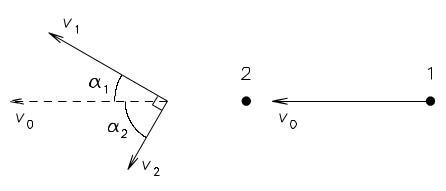
\includegraphics[scale=0.35]{./colision.png}
 % colision.png: 446x191 pixel, 72dpi, 15.73x6.74 cm, bb=0 0 446 191
\end{figure}
\begin{tiny}
 

\begin{eqnarray}
  \bar{p} & = & mv_{s} \left[ 1-4\int_{sen\alpha_{c}}^{1} x^{2} \left( x^{2}-\frac{V^{2}}{v^{2}}(1-x^{2}) \right)^{1/2} dx \right] \approx 0.1 mv_{s} \\
    %n & = & \frac{M_{s}}{m}\frac{\sigma}{m} \rho_{m} v \\
    \frac{d(v-v_{ff})}{dt} & = &  \frac{\bar{p}n}{M_{s}}=\frac{\bar{p}}{m}\frac{\sigma}{m}\rho_{m}v \\
    v-v_{ff} & = & \frac{\bar{p}}{m}\frac{\sigma}{m} \Sigma_{m} \\
    v-v_{ff} &<& 1000 km/s \\
    \frac{\sigma}{m} & < & 7cm^{2}/g
\end{eqnarray}
\end{tiny}
}

\frame{
\begin{itemize}
 \item La supervivencia del c\'umulo secundario.
\end{itemize}
\begin{eqnarray}
 \chi&=&1-2\frac{v^{2}_{esc}}{v_{0}^{2}} \\
   \tau_{m}&=&\frac{\sigma}{m}\Sigma_{m} \\
    \chi \tau_{m}&=&\frac{\sigma}{m}\Sigma_{m} \left[ 1-2 \frac{v_{esc}^{2}}{v_{0}^{2}} \right] \\
    \chi \tau_{m}&<&0.3 \\
     \frac{\sigma}{m}& < &1 cm^{2}/g
\end{eqnarray}

}



\frame{\frametitle{Desafiando la cosmolog\'ia}
\begin{itemize}
 \item Estudio de la probabilidad de que un c\'umulo tenga una velocidad similar a la del bullet cluster. 
    \begin{itemize}
%\begin{tiny}
    \item Hayashi et al. 2006
    \item Farrar y Rosen 2007
    \item Lee y Komatsu 2010
    %\item Forero-Romero et al. 2010
    \item Thompson y Nagamine 2011
    \item Watson et al. 2013
%\end{tiny}
    \end{itemize}
 

 \item Estudios con simulaciones hidrodin\'amicas
    \begin{itemize}
%\begin{tiny}
     \item Springel \& Farrar. 2005
     \item Milosavljevic et al. 2007
     \item Mastropietro \& Burket. 2008
%\end{tiny}
    \end{itemize}

\end{itemize}

}



\section{Mock.}

\frame{
\tableofcontents[ 
    currentsection, 
    hideothersections, 
    sectionstyle=show/hide, 
    sectionstyle=show/shaded, 
    ] 
}

\subsection{Simulaci\'on Millenium}


\frame{\frametitle{Simulaci\'on Millenium}
\begin{figure}[h!]
 \centering
 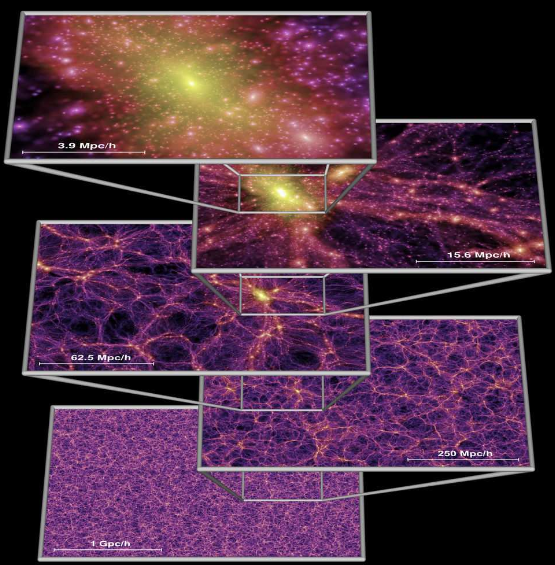
\includegraphics[scale=0.3]{./mill.png}
 % mill.png: 555x565 pixel, 72dpi, 19.58x19.93 cm, bb=0 0 555 565
 \caption{Springel et al. 2005}
\end{figure}

}


\frame{\frametitle{Modelo Cosmol\'ogico $\Lambda CDM$}
\begin{itemize}
 \item $N_{p}=2160^{3} $ \pause
  \item $L=500 Mpc$ \pause
 \item $m_{p}=8.61*10^{8} M_{\odot}$ \pause
 \item $\Omega_{m}=0.25$ ${\color{verde} 0.27 }$ \pause
 \item $\Omega_{b}=0.045$ ${\color{verde} 0.046 }$ \pause
 \item $\Omega_{\Lambda}=0.75$ ${\color{verde} 0.75 }$ \pause
 \item $h=0.73$ $ {\color{verde} 0.72 }$ \pause
 \item $n_{s}=1$ ${\color{verde} 0.99 }$ \pause
 \item $\sigma_{8}=0.9$ ${\color{verde} 0.9 }$ \pause
 \item $Snapshots=64$
\end{itemize}
}

\frame{\frametitle{Estudio de los \'arboles de fusi\'on.}
\begin{itemize}
 \item A partir de los \'arboles de fusi\'on de los subhalos, construimos el \'arbol de fusi\'on del Grupo fof.
\end{itemize}

\begin{figure}[h!]
 \centering
 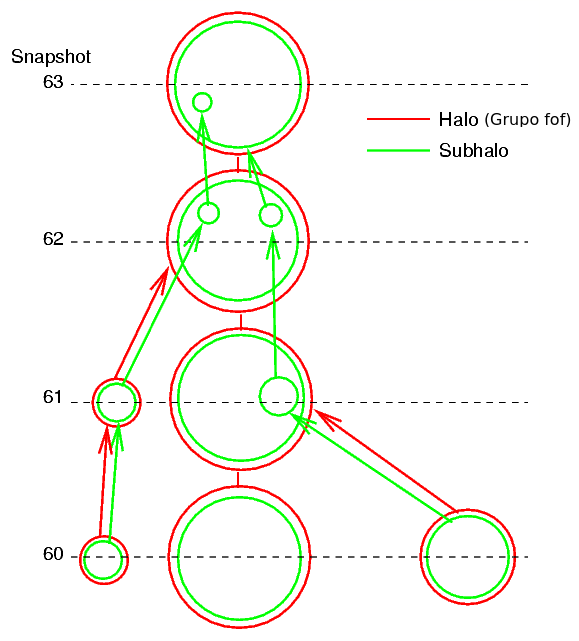
\includegraphics[scale=0.32]{./tree.png}
 % tree.eps: 0x0 pixel, 300dpi, 0.00x0.00 cm, bb=14 14 554 655
\end{figure}

}

\subsection{Modelo semi-anal\'itico: De lucia 2004, Croton et al. 2006}



\frame{\frametitle{Construyendo galaxias: Modelos semi-anal\'itico.}
\begin{itemize}
 \item Cada halo de materia oscura colapsa junto con un conjunto de bariones, siendo la fracci\'on de masa bari\'onica de $f_{b}=17\%$ \pause
 \item Reionizaci\'on: Se utiliza un modelo de 3 fases. \pause 
 \item Para modelar la evoluci\'on de los agujeros negros, se supone que estos crecen durante las fusiones entre galaxias y por la acreci\'on de gas frio,
la cual esta cuantificada por el par\'ametro $f_{BH}$ que representa la fracci\'on de gas frio acretada durante la fusi\'on. \pause
\item Los n\'ucleos activos (AGN) est\'an modelados suponiendo que su actividad es el resultado de la acreci\'on de gas caliente hacia el agujero negro
supermasivo y esta cuantificada por el par\'ametro $\kappa_{AGN}$ que representa la eficiencia de dicha acreci\'on.

\end{itemize}

}

\frame{
\begin{itemize}
 \item Para la fomarci\'on estelar se asume que todas las estrellas se forman en discos de gas fr\'io.
 Luego se calcula una masa cr\'itica y cuando la masa de gas de una galaxia supera dicha masa cr\'itica, la tasa de formaci\'on estelar es:
 $\dot{m}_{*}=\alpha_{sf}(m_{cold}-m_{crit})/t_{dyn,disk}$ \pause
  \item Feedback de supernovas: Estos eventos inyectan gas, metales y energ\'ia en el medio intergal\'actico y pueden calentar el gas fr\'io
 inhibiendo la formaci\'on estelar. Estos fen\'omenos est\'an cuantificados por $\epsilon_{dis}$, $\epsilon_{hal}$ y
$\gamma_{ej}$, donde el primero hace referencia a la eficiencia de la supernova para recalentar el gas frio en el disco, el segundo
es la eficiencia con la cual la supernova eyecta el gas del halo hacia el medio intergal\'actico y el \'ultimo cuantifica la eficiencia
con la cual el gas eyectado por la supernova es reincorporado.

\end{itemize}

}


\frame{\frametitle{Cat\'alogo simulado}
\begin{figure}[h!]
 \centering
 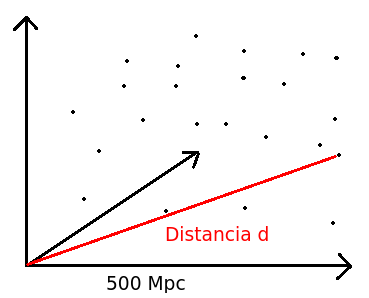
\includegraphics[scale=0.3]{./mock.png}
 % mock.png: 371x289 pixel, 72dpi, 13.09x10.20 cm, bb=0 0 371 289
\end{figure}
\begin{columns}
\begin{column}{5.2cm}
\begin{itemize}
 \item $v_{r}=H_{0}*d+\vec{v_{pec}}\cdot\vec{x}$ \pause
 \item $z=\frac{v_{r}}{c}$ \pause
 \item $D_{M}=c\int_{0}^{z} H(z\prime)dz\prime$ \pause
 \item $D_{L}=D_{M}(1+z)$ \pause

\end{itemize}
\end{column}
\begin{column}{4cm}
 \begin{itemize}
  \item $DM=5LOG(\frac{DL}{10 Pc})$ \pause
  \item $m=M+DM+K$ \pause
  \item $\alpha=atan(\frac{y}{x})$ \pause
  \item $\delta=atan(\frac{z}{\sqrt{x^{2}+y^{2}}})$ \pause
 \end{itemize}

\end{column}

\end{columns}
Este cat\'alogo fue realizado sobre toda la esfera ($4 \pi$) sin utilizar ninguna m\'ascara.
}

\frame{
\frametitle{Cat\'alogo simulado}
\begin{columns}
 \begin{column}{4.2cm}
  \begin{figure}[h!]
 \centering
 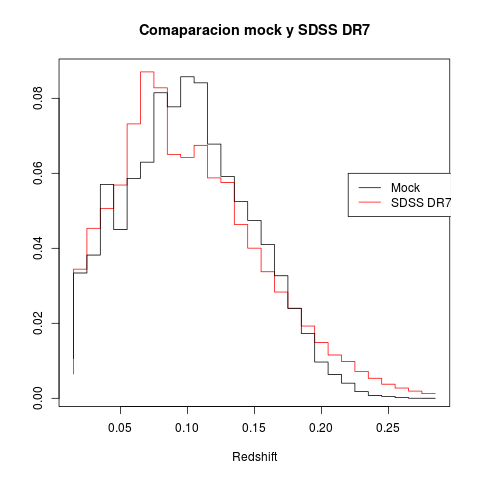
\includegraphics[scale=0.31]{./comparacion_red.png}
 % comparacion_red.png: 480x480 pixel, 72dpi, 16.93x16.93 cm, bb=0 0 480 480
\end{figure}
 \end{column}
 \begin{column}{5cm}
  \begin{figure}[h!]
 \centering
 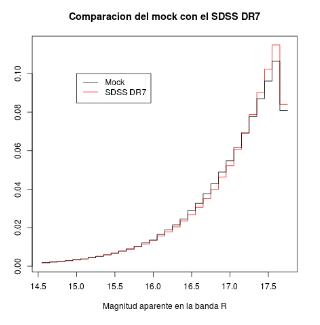
\includegraphics[scale=0.45]{./nu.png}
 % comaracion_bandar.png: 480x480 pixel, 72dpi, 16.93x16.93 cm, bb=0 0 480 480
\end{figure}
 \end{column}
\end{columns}
}



\section{Test de identificaci\'on de subestructuras.}
\frame{
\tableofcontents[ 
    currentsection, 
    hideothersections, 
    sectionstyle=show/hide, 
    sectionstyle=show/shaded, 
    ] 
}

\subsection{Test de Dressler-Shectman}
\frame{\frametitle{Test de Dressler-Shectman}
\begin{itemize}
 \item Se define el estad\'istico: $\delta^{2}=(\frac{11}{\sigma^{2}})[(v_{local}-v)^{2}+(\sigma_{local}-\sigma)^{2}]$
donde \pause
 \item $v$: Velocidad media del c\'umulo. \pause
 \item $v_{local}$: Velocidad media local. Se tienen en cuenta las 10 galaxias m\'as cercanas. \pause
 \item $\sigma$: Dispersi\'on de velocidades del c\'umulo. \pause
 \item $\sigma_{local}$: Dispersi\'on de velocidades local. \pause
 \item Se define el estad\'istico: $\Delta=\Sigma\delta$. \pause
 \item \textit{Pinkney et al.} 
  

  \begin{itemize}
 \begin{tiny}
   \item Es el mejor test de identificaci\'on de subestructuras.
   \item La tasa de efectividad baja cuando las subestructuras est\'an a lo largo de la l\'inea de la visual y cuando el c\'umulo tiene menos de 30 galaxias.
 \item Recomiendan complementar este test con la medici\'on de la Skewness de la distribuci\'on de velocidades radiales.
 \item Puede identificar las subsestructuras provenientes de una fusi\'on hasta 3 Gyr despu\'es de dicha
 interacci\'on, lo que equivale a 10 snapshots en la simulaci\'on, es decir, hasta el snapshot 53.
 \end{tiny}
  \end{itemize}
\end{itemize}
}


\frame{
\begin{itemize}
 \item Como no se conoce la distribuci\'on del estad\'istico $\Delta$, es necesario correr realizaciones Monte Carlo
 distribuyendo aleatoriamente la velocidad, de manera de borrar la subestructuras manteniendo la distribuci\'on de velocidades. \pause
 \item Definimos el valor p mediante
 
 \begin{equation}
  p=\frac{N(\Delta_{MC}> \Delta)}{N_{MC}}
 \end{equation}

\end{itemize}


}

%\begin{frame}[plain]
%\begin{block}{C\'umulo sin subestructura.}
 %\begin{columns}
  %\begin{column}{2cm}
   %\begin{figure}[h!]
    %\centering
    %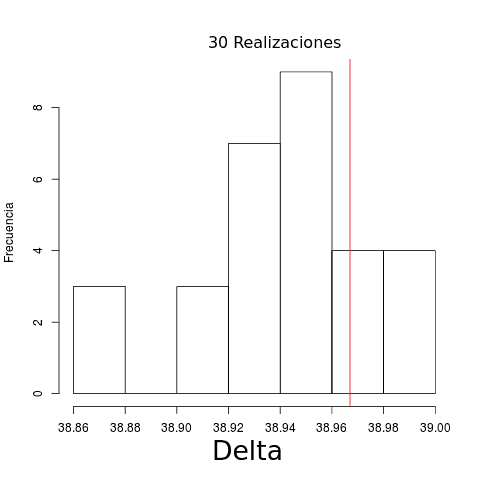
\includegraphics[scale=0.25]{./71_30.png}
 % 71_30.png: 480x480 pixel, 72dpi, 16.93x16.93 cm, bb=0 0 480 480
   %\end{figure}
  %\end{column} 
 % \begin{column}{2cm}
  % \begin{figure}[h!]
   % \centering
    % 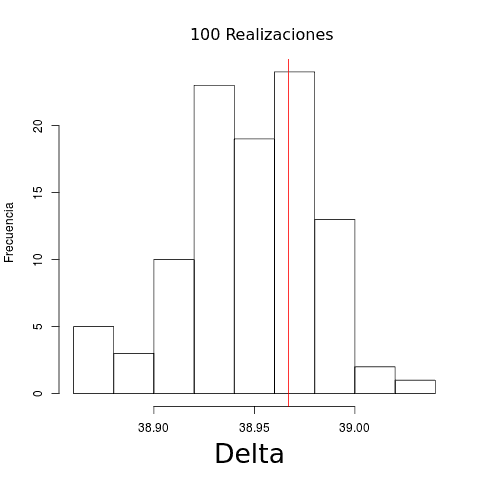
\includegraphics[scale=0.25]{./71_100.png}
 % 71_100.png: 480x480 pixel, 72dpi, 16.93x16.93 cm, bb=0 0 480 480
   %\end{figure}
 % \end{column}
 % \begin{column}{2cm}
  % \begin{figure}[h!]
   % \centering
   % 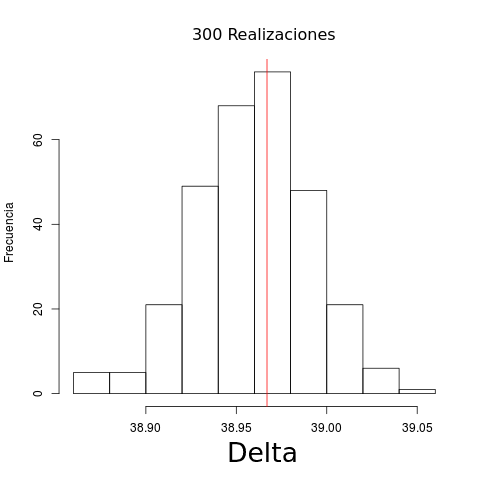
\includegraphics[scale=0.25]{./71_300.png}
 % 71_300.png: 480x480 pixel, 72dpi, 16.93x16.93 cm, bb=0 0 480 480
  % \end{figure}
  %\end{column}
 %\end{columns}
%\end{block}

%\begin{block}{C\'umulo con subestructura.}
% \begin{columns}
%  \begin{column}{2cm}
 %  \begin{figure}[h!]
  %  \centering
   % 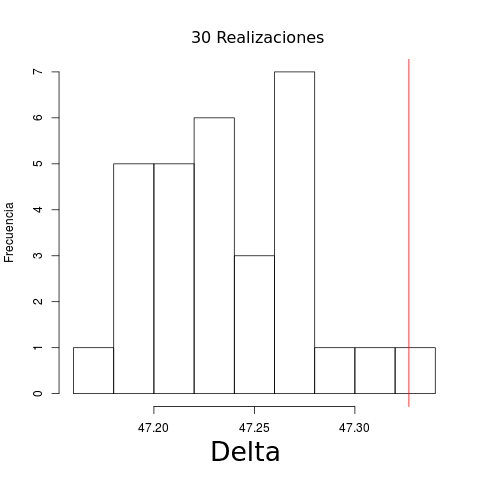
\includegraphics[scale=0.22]{./147_30.png}
 % 147_30.png: 480x480 pixel, 72dpi, 16.93x16.93 cm, bb=0 0 480 480
  % \end{figure}
 % \end{column}
 % \begin{column}{2cm}
  % \begin{figure}[h!]
   % \centering
   % 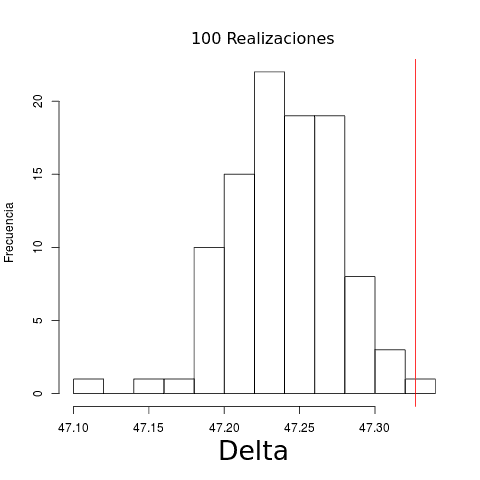
\includegraphics[scale=0.22]{./147_100.png}
 % 147_100.png: 480x480 pixel, 72dpi, 16.93x16.93 cm, bb=0 0 480 480
  % \end{figure}
 % \end{column}
 % \begin{column}{2cm}
  % \begin{figure}[h!]
   % \centering
   % 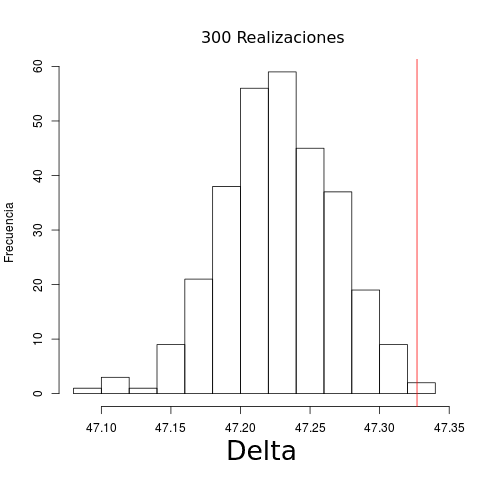
\includegraphics[scale=0.22]{./147_300.png}
 % 147_300.png: 480x480 pixel, 72dpi, 16.93x16.93 cm, bb=0 0 480 480
  % \end{figure}
 % \end{column}
 %\end{columns}
%\end{block}

%\end{frame}


\frame{
\begin{columns}
 \begin{column}{4cm}
  \begin{figure}[h!]
 \centering
 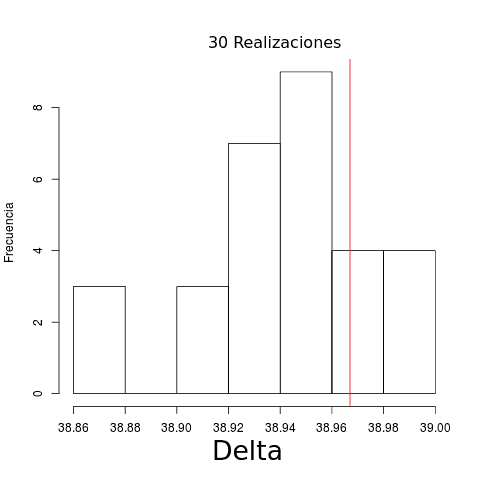
\includegraphics[scale=0.28]{./71_30.png}
 % 71_30.png: 480x480 pixel, 72dpi, 16.93x16.93 cm, bb=0 0 480 480
\end{figure}
\begin{figure}[h!]
 \centering
 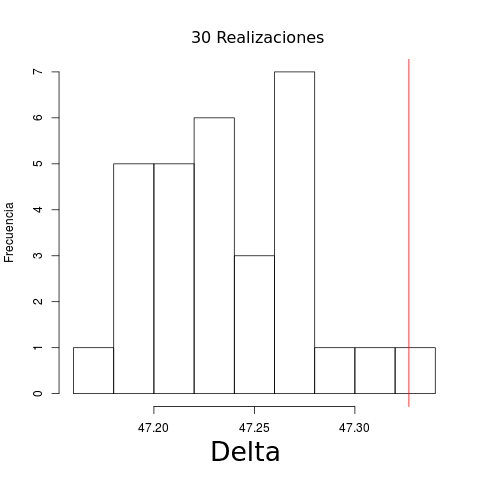
\includegraphics[scale=0.28]{./147_30.png}
 % 147_30.png: 480x480 pixel, 72dpi, 16.93x16.93 cm, bb=0 0 480 480
\end{figure}
 \end{column}
 \begin{column}{4cm}
  \begin{figure}[h!]
 \centering
 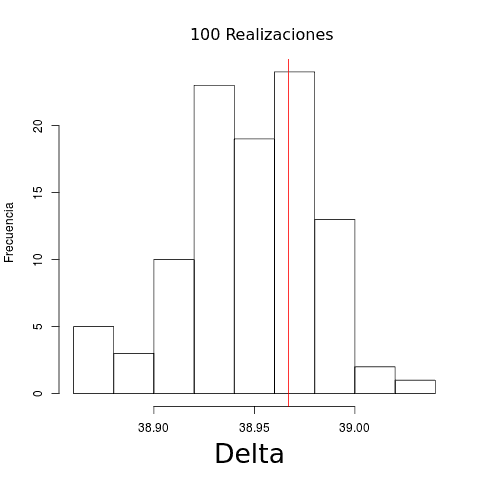
\includegraphics[scale=0.28]{./71_100.png}
 % 71_100.png: 480x480 pixel, 72dpi, 16.93x16.93 cm, bb=0 0 480 480
\end{figure}
\begin{figure}[h!]
 \centering
 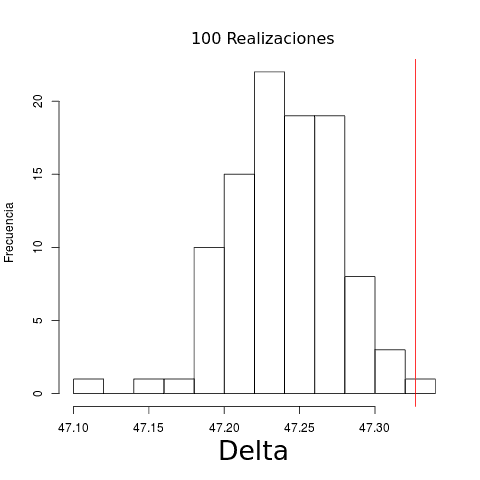
\includegraphics[scale=0.28]{./147_100.png}
 % 147_100.png: 480x480 pixel, 72dpi, 16.93x16.93 cm, bb=0 0 480 480
\end{figure}
 \end{column}
\begin{column}{4cm}
 \begin{figure}[h!]
 \centering
 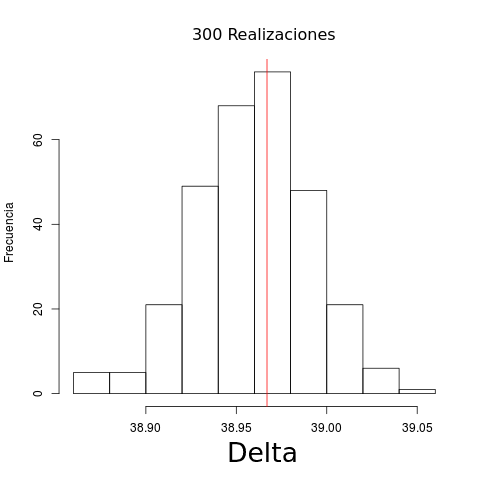
\includegraphics[scale=0.28]{./71_300.png}
 % 71_300.png: 480x480 pixel, 72dpi, 16.93x16.93 cm, bb=0 0 480 480
\end{figure}
\begin{figure}[h!]
 \centering
 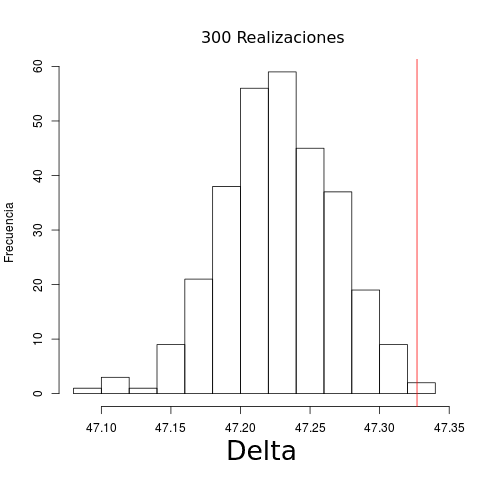
\includegraphics[scale=0.28]{./147_300.png}
 % 147_300.png: 480x480 pixel, 72dpi, 16.93x16.93 cm, bb=0 0 480 480
\end{figure}
\end{column}
\end{columns}

}

\subsection{Test de Dressler-Shectman iterativo.}
\frame{\frametitle{Test de Dressler-Shectman iterativo} 
\begin{itemize}
 \item $\delta^{2}=(\frac{0.2*ngal}{\sigma^{2}})[(v_{local}-v)^{2}+(\sigma_{local}-\sigma)^{2}]$ \pause
 \item Se elminan aquellas galaxias con $\delta<0.7 \bar{\delta}$ \pause
 \item Se calcula nuevamente $\delta^{2}=(\frac{0.2*ngal}{\sigma^{2}})[(v_{local}-v)^{2}+(\sigma_{local}-\sigma)^{2}]$ \pause
 \item Decimos que el algoritmo converge si el n\'umero de galaxias entre 2 pasos consecutivos es igual.
\end{itemize}
}
\frame{
\begin{figure}[h!]
 \centering
 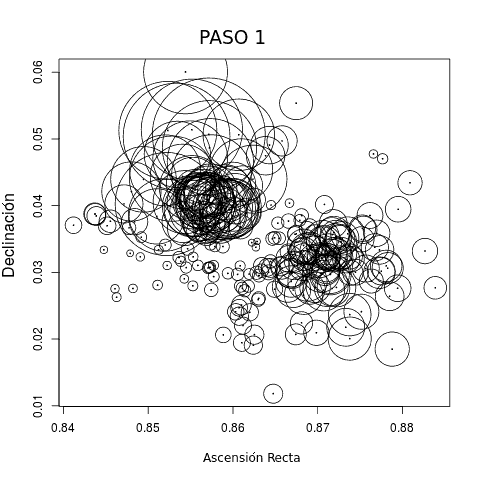
\includegraphics[scale=0.3]{./dlr11.png}
 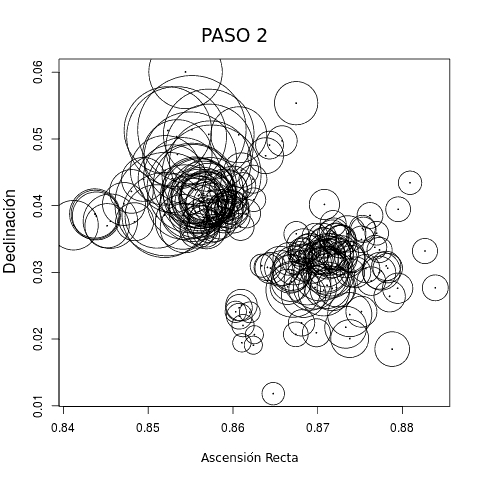
\includegraphics[scale=0.3]{./dlr21.png}
 \end{figure}
 
 \begin{figure}
 \centering 
  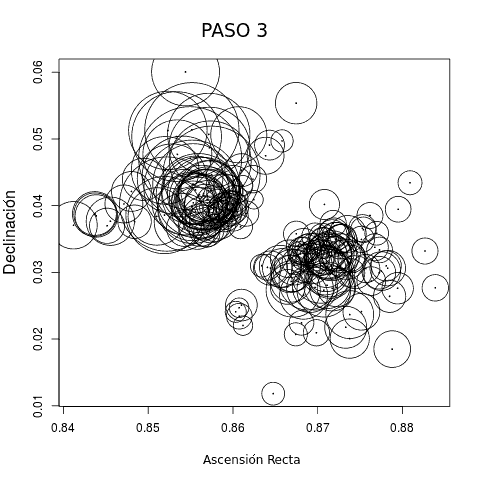
\includegraphics[scale=0.3]{./dlr31.png}
 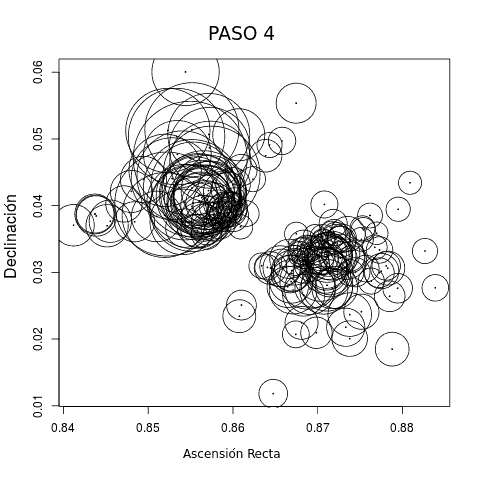
\includegraphics[scale=0.3]{./dlr41.png}
 % dlr1.png: 480x480 pixel, 72dpi, 16.93x16.93 cm, bb=0 0 480 480

\end{figure}

}



\subsection{Mixtura de gaussianas.}
\frame{\frametitle{Mixtura de gaussianas (\textit{Mclust})}
Dado que la aplicaci\'on del test de DS nos deja un conjunto de galaxias con alta probabilidad
de residir en subestructuras, resulta necesario agrupar las mismas con el fin de definirlas y establecer
sus propiedades f\'isicas.


\begin{figure}[h!]
 \centering
 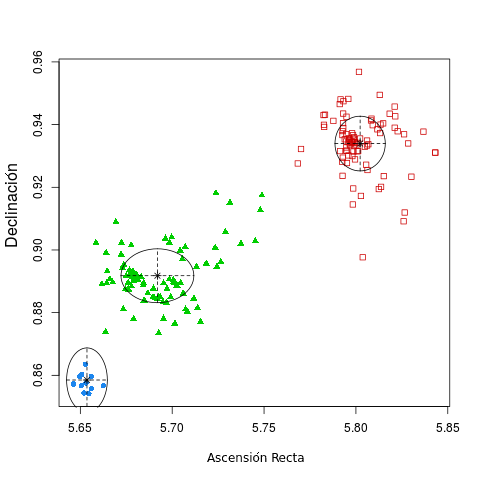
\includegraphics[scale=0.28]{./mclust_class.png}
 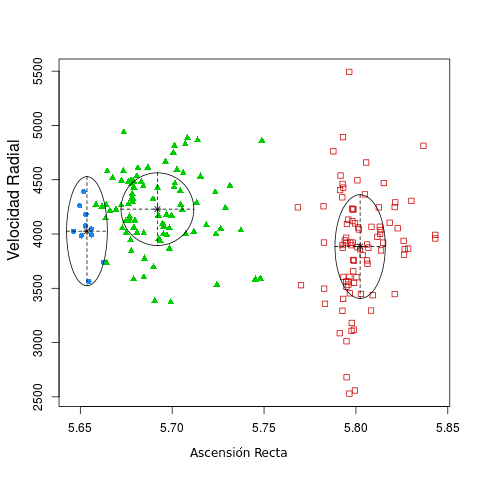
\includegraphics[scale=0.28]{./mclust_13.png}
 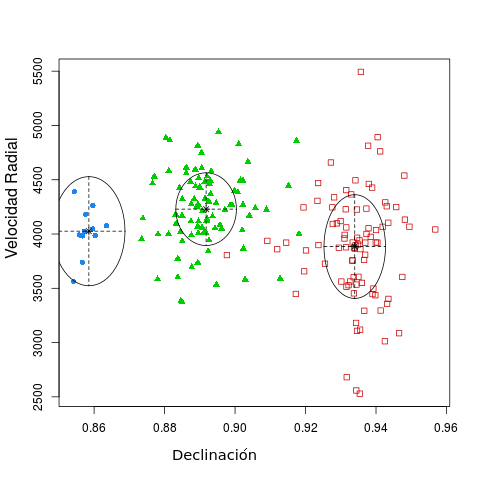
\includegraphics[scale=0.28]{./mclust_23.png}
 % mclust_class.png: 480x480 pixel, 96dpi, 12.70x12.70 cm, bb=0 0 360 360

\end{figure}

}


\frame{\frametitle{Aplicaci\'on del Test de DS en el cat\'alogo simulado}
\begin{itemize}
\item Aplicamos el test a 2854 c\'umulos con masas mayores a $10^{13}M_{\odot}$ y con m\'as de 30 galaxias. \pause
\item Encontramos que 1448 c\'umulos presentan subestructuras ($p<0.15$), lo que representa aproximadamente un $50 \%$ de la muestra. \pause
\item Si adem\'as pedimos que la Skewness de la distribuci\'on de velocidades radiales sea distinta a 0, la muestra se reduce a 715 c\'umulos.
\end{itemize}
}
\frame{
\begin{figure}[h!]
 \centering
  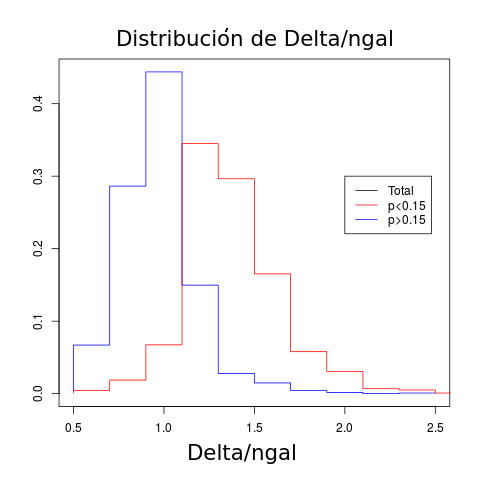
\includegraphics[scale=0.4]{./histdeltas.png}
 % hist.deltas4pi.png: 480x480 pixel, 72dpi, 16.93x16.93 cm, bb=0 0 480 480
 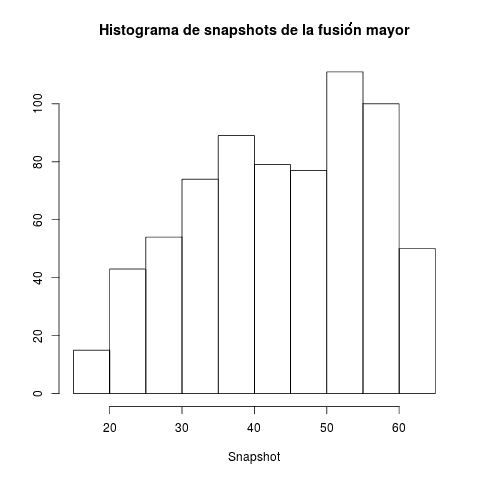
\includegraphics[scale=0.4]{./hist_snap1.png}


\end{figure}

}

\frame{\frametitle{Aplicaci\'on del test de DS iterativo}
\begin{itemize}
 \item Aplicamos el test de DS iterativo a los 2854 c\'umulos de la muestra y encontramos que en 119, el test converge. \pause
 \item De estos 119, solo 46 tambi\'en fueron detectados por el test de DS tradicional complementado con el test de Skewnes.
\end{itemize}

\begin{figure}[h!]
 \centering
 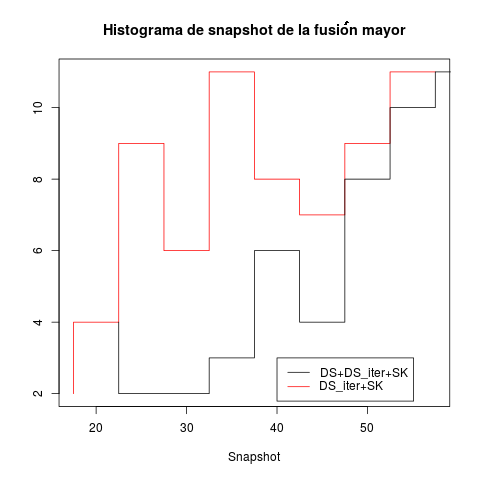
\includegraphics[scale=0.4]{./hist_snap_todo.png}

\end{figure}

}


\frame{\frametitle{Aplicaci\'on de la mixtura de gaussianas.}
\begin{itemize}
 \item Utilizamos el programa \textit{Mclust} sobre aquellas galaxias con $\delta > 2$. \pause
 \item En 636 c\'umulos, de la muestra de 715 c\'umulos, se encuentran 2 subestructuras. \pause
 \item Econtramos que en 44 de los 46 c\'umulos, de la muestra identificada por ambos test de DS m\'as el test de Skewness, hay 2 subestructuras
 significativas.
\end{itemize}

}

\frame{
%\begin{columns}
%\begin{column}{5cm}
\begin{figure}[h!]
 \centering
 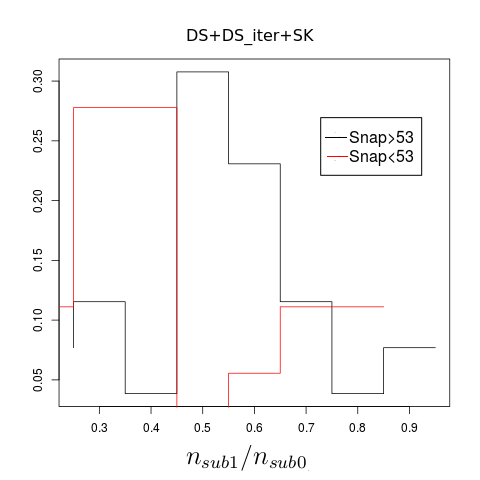
\includegraphics[scale=0.3]{./hist_mclus_numrel_dsiter.png}
  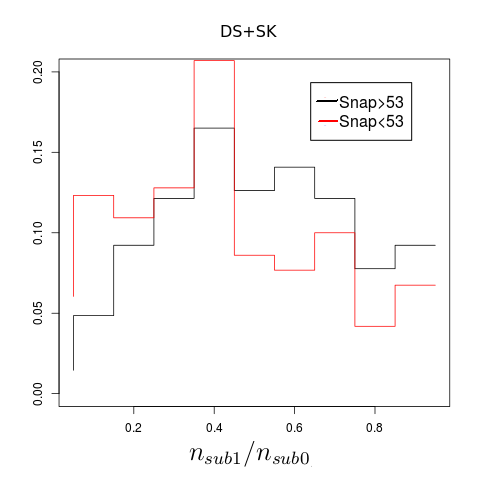
\includegraphics[scale=0.3]{./hist_mclus_numrel.png}
%\end{figure}
%\end{column}

%\begin{column}{4cm}
%\begin{figure}[h!]
% \centering
 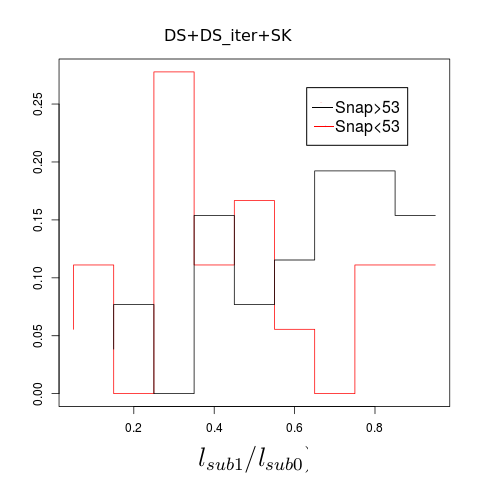
\includegraphics[scale=0.3]{./hist_mclus_lumrel_dsiter.png}
 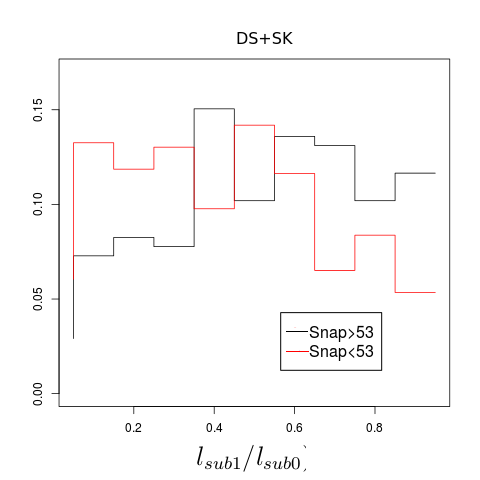
\includegraphics[scale=0.3]{./hist_mclus_lumrel.png}
\end{figure}
%\end{column}
%\end{columns}
}

\frame{
\begin{itemize}
 \item De los 715 c\'umulos, 190 presentan una ocupaci\'on relativa mayor a 0.5. \pause
 \item De los 46 c\'umulos, 20 presentan una ocupaci\'on relativa mayor a 0.5.
\end{itemize}

\begin{figure}[h!]
 \centering
 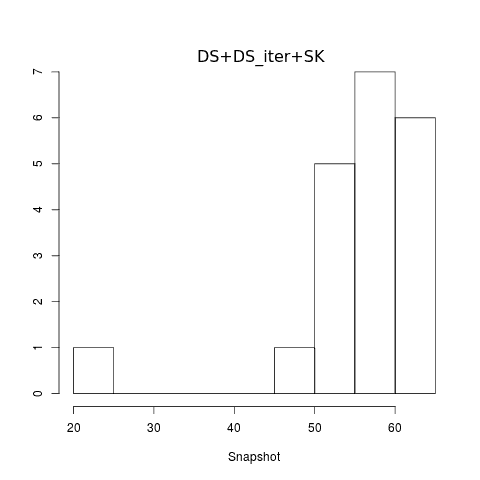
\includegraphics[scale=0.45]{./hist_snap_mclust_dsiter.png}
 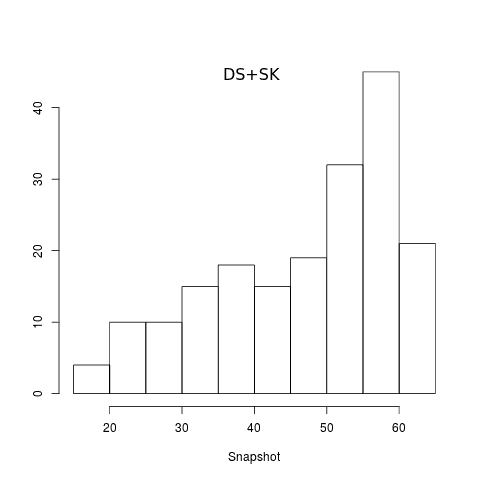
\includegraphics[scale=0.45]{./hist_snap_mclust_ds.png}

\end{figure}
}

\frame{\frametitle{Estudio de las subestructuras identificadas.}
\begin{tiny}
 

\begin{itemize}
\item Luego de la identificaci\'on de la subestructuras de esta muestra, cada una de estas fue asociada con un halo del mock, teniendo en cuenta cual era el halo del mock
con mayor cantidad de galaxias en dicha subestructura encontrada por el programa \textit{mclust}. \pause
 \item Para lograr una mejor identificaci\'on de las subestructuras, calculamos las coordenadas del centro, pesadas por luminosidad. \pause
 \item Luego estimamos la dispersi\'on de velocidades y el radio virial mediante:
 
\begin{eqnarray} \label{rvir_disp}
 R_{vir} & = & \frac{\pi}{2} \frac{ngal(ngal-1)}{\sum_{i>j}^{ngal}R_{ij}^{-1}} \nonumber\\
 \sigma &=& \frac{\sqrt{\pi}}{ngal(ngal-1)} \sum_{i=1}^{ngal-1} \omega_{i} g_{i} \nonumber\\
 \omega_{i} &=& i(ngal-i) \nonumber\\
 g_{i} &=& v_{i+1}-v_{i} \nonumber\\ 
\end{eqnarray}
\end{itemize}
\end{tiny}
}

\frame{\frametitle{Estudio de las subestructuras identificadas.}
%\begin{tiny}
 

\begin{itemize}
%\item Luego de la identificaci\'on de la subestructuras de esta muestra, cada una de estas fue asociada con un halo del mock, teniendo en cuenta cual era el halo del mock
%con mayor cantidad de galaxias en dicha subestructura encontrada por el programa \textit{mclust}. 
% \item Para lograr una mejor identificaci\'on de las subestructuras, calculamos las coordenadas del centro, pesadas por luminosidad. 
 \item Comparamos los centros de los grupos identificados, con los centros de los halos asociados, encontrando que nuestra estimaci\'on del 
 centro es buena. \pause
 \item Comparamos los radios viriales de los grupos identificados con los radios viriales de los halos asociados, encontrando que estamos
 sobreestimando dichos radios. \pause
 \item Comparamos la dispersi\'on de velocidad de los grupos identificados con la dispersi\'on de velocidad de los halos asociados, encontrando
 que nuestro c\'alculo es una buena estimaci\'on de dicho valor.

\end{itemize}
%\end{tiny}
}

%\frame{

%\begin{columns}
% \begin{column}{5cm}
%\begin{figure}[h!]
% \centering
% 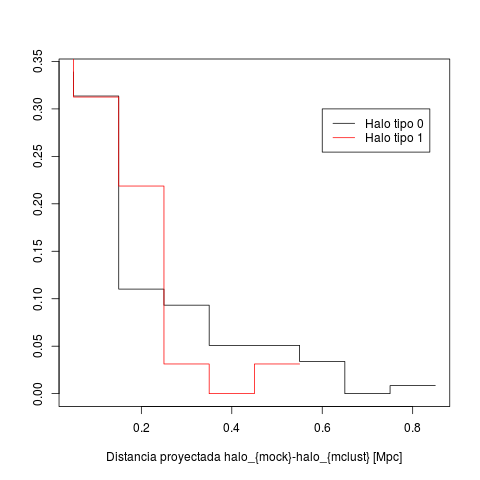
\includegraphics[scale=0.35]{./histo_dist_mock_mclus.png}
%\end{figure}
% \end{column}
% \begin{column}{5cm}
%\begin{figure}[h!]
% \centering
% 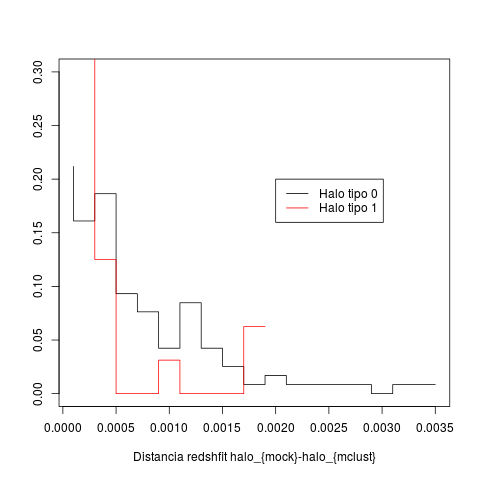
\includegraphics[scale=0.35]{./histo_distred_mock_mclus.png}
%\end{figure}
% \end{column}
%\end{columns}

%}


%\frame{
%\begin{columns}
% \begin{column}{5cm}
%\begin{figure}[h!]
% \centering
% 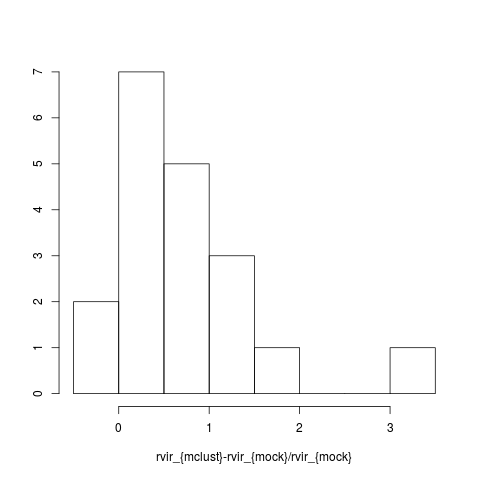
\includegraphics[scale=0.35]{./rvirrvir.png}
%\end{figure}
% \end{column}
% \begin{column}{5cm}
%\begin{figure}[h!]
% \centering
% 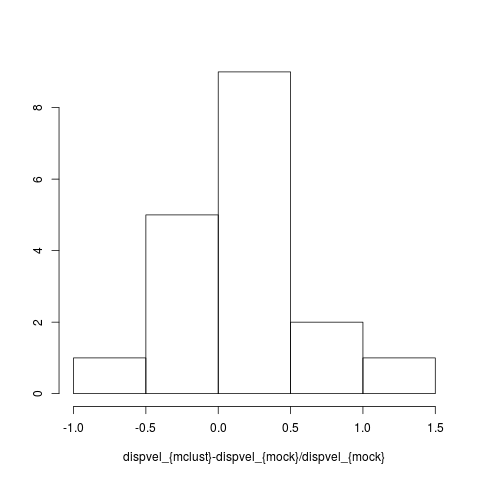
\includegraphics[scale=0.35]{./dispvelvel.png}
 % histo_dif_dispvel.png: 480x480 pixel, 72dpi, 16.93x16.93 cm, bb=0 0 480 480
%\end{figure}
% \end{column}
%\end{columns}
%}

\frame{

\begin{columns}
 \begin{column}{5cm}
\begin{figure}[h!]
 \centering
 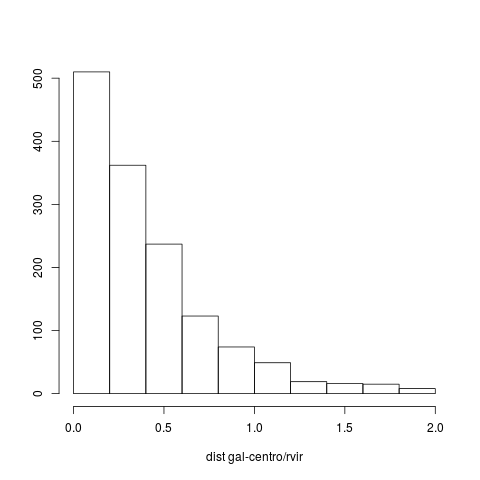
\includegraphics[scale=0.35]{./histo_dist_gal_centro.png}
\end{figure}
 \end{column}
 \begin{column}{5cm}

\begin{figure}[h!]
 \centering
  \includegraphics[scale=0.35]{./histo_distvel_gal_centro.png}
\end{figure}
 \end{column}
\end{columns}
}

\frame{
\begin{itemize}
 \item Consideramos miembros de un grupo solamente aquellas galaxias que se encuentran a una distancia
proyectada menor que el radio virial $r_{vir}$ y con una diferencia de velocidades radiales menor a $2\sigma$.

\end{itemize}
\begin{figure}[h!]
 \centering
 \includegraphics[scale=0.35]{./puto.png}
\end{figure}
}

\frame{

Al realizar la asociaci\'on entre grupos identificados por \textit{mclust} y subhalos del mock encontramos 3 casos:

\begin{enumerate}
 \item C\'umulos en el que identificamos el subhalo tipo 0 (subhalo principal del grupo fof) y un subhalo tipo 1. \pause
 \item C\'umulos en los que identificamos dos subhalos tipo 1. \pause
 \item C\'umulos en los que el programa \textit{mclust} encuentra dos grupos que est\'an asociados a un solo subhalo tipo 0 en el mock. \pause
\end{enumerate}

De los 715 c\'umulos, en 28 encontramos 2 subestructuras con una ocupaci\'on relativa mayor a $0.5$ y cuyos grupos tengan m\'as de 3 galaxias. 
 De estos 28, en 19 encontramos el halo tipo 0 y un halo tipo 1 (caso 1), en 4 encontramos 2 halos 
tipo 1 (caso 2) y en 5 se genera una falsa subestructura a partir del ajuste de las gaussianas (caso 3).
}

%\frame{
%\begin{figure}[h!]
% \centering
% \includegraphics[scale=0.23]{./casolindo100.png}
% \includegraphics[scale=0.23]{./casolindo5.png}
% \includegraphics[scale=0.23]{./casolindo103.png}
%\end{figure}
%}

\frame{
\begin{figure}[h!]
 \centering
 \includegraphics[scale=0.34]{./histo_arribo.png}
 \includegraphics[scale=0.34]{./histo_masarel_mock.png}

\end{figure}

}
%\frame{
%\begin{figure}[h!]
% \centering
% \includegraphics[scale=0.5]{./grafico_chala.png}
%\end{figure}
%}

\frame{
A partir de la asociaci\'on entre grupos identificados con \textit{mclust} y subhalos del mock, se pueden definir 3 par\'ametros para evaluar dichas subestructuras.
\begin{enumerate}
 \item Completitud: La completitud esta definida como el n\'umero de galaxias del grupo encontrado por \textit{mclust} que pertenecen al subhalo
 asociado, divido la cantidad de galaxias del subhalo asociado. \pause
 \item Contaminaci\'on: La contaminaci\'on es la cantidad de galaxias del grupo encontrado por \textit{Mclust} que no pertenecen al subhalo asociado,
 dividido la cantidad de galaxias del subhalo asociado. \pause
 \item Pureza: La pureza es la cantidad de galaxias del subhalo asociado, divido la cantidad de galaxias del grupo encontrado.
\end{enumerate}
}

\frame{
\begin{figure}[h!]
 \centering
 \includegraphics[scale=0.45]{./compl_binmasa_02.png}
  \includegraphics[scale=0.45]{./compl_binnum_tipo1.png}
\end{figure}

}
\frame{
\begin{figure}[h!]
 \centering
 \includegraphics[scale=0.45]{./cont_binmasa_02.png}
  \includegraphics[scale=0.45]{./cont_binnum_tipo1.png}
\end{figure}

}
\frame{
\begin{figure}[h!]
 \centering
 \includegraphics[scale=0.45]{./pur_binmasa_02.png}
  \includegraphics[scale=0.45]{./pur_binnum_tipo1.png}
\end{figure}

}


%------------------------------------------------------------------------------------------------------------------------------------------------
%------------------------------------------------------------------------------------------------------------------------------------------------
%------------------------------------------------------------------------------------------------------------------------------------------------
%------------------------------------------------------------------------------------------------------------------------------------------------
%------------------------------------------------------------------------------------------------------------------------------------------------
%------------------------------------------------------------------------------------------------------------------------------------------------
%------------------------------------------------------------------------------------------------------------------------------------------------
\section{Resultados.}
\frame{
\tableofcontents[ 
    currentsection, 
    hideothersections, 
    sectionstyle=show/hide, 
    sectionstyle=show/shaded, 
    ] 
}

\subsection{Cat\'alogo de grupos y c\'umulos de galaxias del SDSS DR3.}
\frame{\frametitle{Aplicaci\'on del m\'etodo de detecci\'on: Cat\'alogo de \textit{Berlind. et al}}
\begin{tiny}
 

\begin{itemize}
 \item Contiene informaci\'on sobre 8148 c\'umulos y grupos de galaxias, que representan una muestra de 44554 galaxias. \pause
 \item Este cat\'alogo fue realizado utilizando un algoritmo \textit{Friend-of-Friends (FOF)}, sobre 3 muestras limitadas por vol\'umen del cat\'alogo de galaxias
SDSS DR3. \pause
\item Solo 77 c\'umulos tienen una ocupaci\'on mayor a 30. \pause
\item Encontramos que $30$ c\'umulos presentan subestructura significativa ($pval<0.15$), 
representando el $40\%$ de la muestra aproximadamente, valor similar a los encontrados en trabajos anteriores (\textit{Geller et al.}, 
\textit{Dressler et al.} y \textit{West et al.}). \pause
\item Todos estos c\'umulos presentan una skewness de la distribuci\'on de velocidades radiales distinta de $0$.\pause
\item De estos 30 c\'umulos, 20 presentan subestructura seg\'un el test de DS iterativo.\pause
\item Identificamos las subestructuras presentes en los c\'umulos previamente seleccionados, a trav\'es del programa \textit{mclust}, corrido
sobre todas las galaxias con $\delta>2$, encontrando 2 subestructuras significativas en $15$ de los c\'umulos de la muestra.
\end{itemize}
\end{tiny}
}


%\frame{
%\begin{figure}[h!]
% \centering
% \includegraphics[scale=0.4]{./dist_centros_comp_ber.png}
% \includegraphics[scale=0.4]{./distvel_centros_comp_ber.png}
%\end{figure}
%}


\subsection{Cat\'alogo de grupos y c\'umulos de galaxias del SDSS DR8.}
\frame{\frametitle{Aplicaci\'on del m\'etodo de detecci\'on: Cat\'alogo de \textit{Tempel et al.}}
\begin{tiny}
 

\begin{itemize}
 \item Contiene informaci\'on sobre 77858 c\'umulos y grupos de galaxias, que representan una muestra de 576493 galaxias.\pause
\item Fue realizado utilizando un algoritmo FOF modificado con una longitud de linkeo variable seg\'un el redshift, aplicado sobre el 
SDSS DR8 , para galaxias con una magnitud aparente en la banda r de hasta $17.77$.\pause
\item Al igual que en el cat\'alogo de \textit{Berlind et al.}, solamente $389$ c\'umulos tienen una ocupaci\'on mayor a 30.\pause
\item Encontramos que $246$ c\'umulos presentan subestructura significativa ($pval<0.15$).\pause
\item Si adem\'as pedimos que la skewness de la distribuci\'on de velocidades radiales sea distinta de 0, la muestra se reduce a $132$.\pause
\item De estos $132$ c\'umulos, $86$ presentan subestructura seg\'un el test de DS iterativo.\pause
\item Identificamos las subestructuras presentes en los c\'umulos previamente seleccionados, a trav\'es del programa \textit{mclust}, corrido
sobre todas las galaxias con $\delta>2$, encontrando 2 subestructuras significativas en $80$ de los c\'umulos de la muestra.
\end{itemize}
\end{tiny}
}

%\frame{
%\begin{figure}[h!]
% \centering
% \includegraphics[scale=0.4]{./dist_centros_com_tem.png}
% \includegraphics[scale=0.3]{./distvel_centros_com_tem.png}
%\end{figure}
%}

\subsection{Cat\'alogo de grupos y c\'umulos de galaxias del 2DF.}
\frame{\frametitle{Aplicaci\'on del m\'etodo de detecci\'on: Cat\'alogo de \textit{Eke et al.}}
\begin{tiny}
 

\begin{itemize}
 \item Contiene informaci\'on sobre 28877 c\'umulos y grupos de galaxias, que representan una muestra de 191440 galaxias.\pause
\item Fue realizado utilizando un algoritmo FOF modificado con una longitud de linkeo variable seg\'un el redshift y la densidad 
de galaxias, aplicado sobre el 2Df.\pause
\item Solamente $144$ c\'umulos tienen una ocupaci\'on mayor a 30.\pause
\item Encontramos que $112$ c\'umulos presentan subestructura significativa ($pval<0.15$).\pause
\item Si adem\'as pedimos que la skewness de la distribuci\'on de velocidades radiales sea distinta de 0, la muestra se reduce a $60$.\pause
\item De estos $60$ c\'umulos, $41$ presentan subestructura seg\'un el test de DS iterativo.\pause
\item Identificamos las subestructuras presentes en los c\'umulos previamente seleccionados, a trav\'es del programa \textit{mclust}, corrido
sobre todas las galaxias con $\delta>2$, encontrando 2 subestructuras significativas en $38$ de los c\'umulos de la muestra.
\end{itemize}
\end{tiny}
}


%\frame{
%\begin{figure}[h!]
% \centering
% \includegraphics[scale=0.4]{./dist_centros_comp_2df.png}
% \includegraphics[scale=0.4]{./distvel_centros_comp_2df.png}
%\end{figure}
%}

%\subsection{Comparaci\'on con otros resultados.}
%\frame{\frametitle{Comparaci\'on con otros resultados.}

%}
%------------------------------------------------------------------------------------------------------------------------------------------------
%------------------------------------------------------------------------------------------------------------------------------------------------
%------------------------------------------------------------------------------------------------------------------------------------------------
%------------------------------------------------------------------------------------------------------------------------------------------------
%------------------------------------------------------------------------------------------------------------------------------------------------
%------------------------------------------------------------------------------------------------------------------------------------------------
%------------------------------------------------------------------------------------------------------------------------------------------------

\section{Conclusiones}
\frame{
\tableofcontents[ 
    currentsection, 
    hideothersections, 
    sectionstyle=show/hide, 
    sectionstyle=show/shaded, 
    ] 
}

\frame{\frametitle{Resumen.}
\begin{itemize}
\item Se construyo un cat\'alogo simulado de galaxias.\pause
\item Se construyo un \'arbol de fusi\'on para los grupos fof.\pause
\item Se estudiaron diferentes m\'etodos para la identificaci\'on de subestructuras, entre ellos, uno desarrollado por nosotros.\pause
\item Se estudiaron los \'arboles de fusi\'on de los c\'umulos seleccionados por los diferentes m\'etodos.\pause
\item Se identificaron y estudiaron las subestructuras presentes en dichos c\'umulos, encontrando las galaxias miembros y calculando
sus propiedades f\'isicas m\'as relevantes.\pause
\item Se aplicaron los m\'etodos estudiados a cat\'alogos de galaxias reales, armando una muestra de c\'umulos de galaxias en proceso 
de colisi\'on.
\end{itemize}
}

\frame{\frametitle{Trabajo a futuro}
\begin{itemize}
 \item Explorar variantes que mejoren los m\'etodos utilizados (construcci\'on de mejores cat\'algos de galaxias, desarrollo 
 de nuevos m\'etodos de identificaci\'on de subestructuras, etc.). \pause
 %\item Estudiar nuevos m\'etodos de identificaci\'on de subestructuras. \pause
 \item Calibrar con nuevos cat\'alogos simulados el m\'etodo desarrollado, para su aplicaci\'on en cat\'alogos de mayor profundidad. \pause
 \item Estudiar las propiedades f\'isicas de las galaxias que pertenecen a las subestructuras identificadas. \pause
 \item Realizar pruebas astrof\'isicas sobre los c\'umulos del cat\'alogo para determinar propiedades de la materia oscura.
\end{itemize}


}

\frame{
\begin{figure}[h!]
 \centering
 \includegraphics[scale=0.4]{./gracias.png}
 % gracias.png: 657x518 pixel, 72dpi, 23.18x18.27 cm, bb=0 0 657 518
\end{figure}
}
\end{document}

